%%%%%%%%%%%%%%%%%%%%%%%%%%%%%%%%%%%%%%%%%
% Beamer Presentation
% LaTeX Template
% Version 1.0 (10/11/12)
%
% This template has been downloaded from:
% http://www.LaTeXTemplates.com
%
% License:
% CC BY-NC-SA 3.0 (http://creativecommons.org/licenses/by-nc-sa/3.0/)
%
%%%%%%%%%%%%%%%%%%%%%%%%%%%%%%%%%%%%%%%%%

%----------------------------------------------------------------------------------------
%	PACKAGES AND THEMES
%----------------------------------------------------------------------------------------

\documentclass{beamer}

\mode<presentation> {

% The Beamer class comes with a number of default slide themes
% which change the colors and layouts of slides. Below this is a list
% of all the themes, uncomment each in turn to see what they look like.

%\usetheme{default}
%\usetheme{AnnArbor}
%\usetheme{Antibes}
%\usetheme{Bergen}
%\usetheme{Berkeley}
%\usetheme{Berlin}
%\usetheme{Boadilla}
%\usetheme{CambridgeUS}
%\usetheme{Copenhagen}
%\usetheme{Darmstadt}
%\usetheme{Dresden}
%\usetheme{Frankfurt}
%\usetheme{Goettingen}
%\usetheme{Hannover}
%\usetheme{Ilmenau}
%\usetheme{JuanLesPins}
%\usetheme{Luebeck}
\usetheme{Madrid}
%\usetheme{Malmoe}
%\usetheme{Marburg}
%\usetheme{Montpellier}
%\usetheme{PaloAlto}
%\usetheme{Pittsburgh}
%\usetheme{Rochester}
%\usetheme{Singapore}
%\usetheme{Szeged}
%\usetheme{Warsaw}

% As well as themes, the Beamer class has a number of color themes
% for any slide theme. Uncomment each of these in turn to see how it
% changes the colors of your current slide theme.

%\usecolortheme{albatross}
%\usecolortheme{beaver}
%\usecolortheme{beetle}
%\usecolortheme{crane}
%\usecolortheme{dolphin}
%\usecolortheme{dove}
%\usecolortheme{fly}
%\usecolortheme{lily}
%\usecolortheme{orchid}
%\usecolortheme{rose}
%\usecolortheme{seagull}
%\usecolortheme{seahorse}
%\usecolortheme{whale}
%\usecolortheme{wolverine}

%\setbeamertemplate{footline} % To remove the footer line in all slides uncomment this line
%\setbeamertemplate{footline}[page number] % To replace the footer line in all slides with a simple slide count uncomment this line

%\setbeamertemplate{navigation symbols}{} % To remove the navigation symbols from the bottom of all slides uncomment this line
}

\usepackage{graphicx} % Allows including images
\usepackage{booktabs} % Allows the use of \toprule, \midrule and \bottomrule in tables
\usepackage{multirow}
%----------------------------------------------------------------------------------------
%	TITLE PAGE
%----------------------------------------------------------------------------------------


\title[Exercise 2]{Estimating HRF and covariance structure}

\author{Nora Brackbill and Charles Zheng} % Your name
\institute[Stanford] % Your institution as it will appear on the bottom of every slide, may be shorthand to save space
{Stanford University}
\date{\today} % Date, can be changed to a custom date

\begin{document}

\begin{frame}
\titlepage % Print the title page as the first slide
\end{frame}


\begin{frame}
\frametitle{Estimating HRF and amplitudes}
\begin{itemize}
\item Use one block at a time
\item Code the twelve stimuli as 1-12, the ``null'' signal as 13, and the 6 ``calibration'' signals as 14-19
\item Transform stimuli assignments to a matrix $S$,
dimension of $S$ is $T \times K$, $T$ is the time of time points, $K$ the number of stimuli types
\[
\begin{bmatrix}
1\\0\\0\\0\\3\\\vdots
\end{bmatrix} \rightarrow
S = 
\begin{bmatrix}
1 & 0 & 0 & 0\\
0 & 0 & 0 & 0\\
0 & 0 & 0 & 0\\
0 & 0 & 0 & 0\\
0 & 0 & 1 & 0\\
\vdots & \vdots & \vdots & \vdots
\end{bmatrix}
\]
\end{itemize}
\end{frame}


\begin{frame}
\frametitle{Estimating HRF and amplitudes}
Transform estimated or assumed HRF $h = (h_1,\hdots,h_L)$ to matrix $H(h)$.
Dimension of $H(h)$ is $T \times T$
\[
h = 
\begin{bmatrix}
h_1\\h_2\\h_3\\h_4\\h_5\\\vdots
\end{bmatrix} \rightarrow
H(h) = 
\begin{bmatrix}
h_1 & 0 & 0 & \cdots\\
h_2 & h_1 & 0 & \cdots\\
h_3 & h_2 & h_1 & \cdots\\
h_4 & h_3 & h_2 & \cdots\\
h_5 & h_4 & h_3 & \cdots\\
\vdots & \vdots & \vdots & \vdots
\end{bmatrix}
\]

\end{frame}

\begin{frame}
\frametitle{Estimating amplitudes}

Estimate the stimuli-specific amplitudes $\alpha = (\alpha_1,\hdots,\alpha_K)$ by fitting the model
\[
y \sim H(h) S \alpha  + \text{const}= \begin{bmatrix}
h_1 & 0 & 0 & \cdots\\
h_2 & h_1 & 0 & \cdots\\
h_3 & h_2 & h_1 & \cdots\\
h_4 & h_3 & h_2 & \cdots\\
h_5 & h_4 & h_3 & \cdots\\
\vdots & \vdots & \vdots & \vdots
\end{bmatrix}
\begin{bmatrix}
1 & 0 & 0 & 0\\
0 & 0 & 0 & 0\\
0 & 0 & 0 & 0\\
0 & 0 & 0 & 0\\
0 & 0 & 1 & 0\\
\vdots & \vdots & \vdots & \vdots
\end{bmatrix}
\begin{bmatrix}
\alpha_1\\\alpha_2\\\alpha_3\\\vdots
\end{bmatrix}  + \text{const}
\]

\end{frame}


\begin{frame}
\frametitle{Estimating HRF}
Suppose instead that $\alpha$ is known and $h$ is unknown.  Then let $t = S\alpha = (t_1,t_2,\hdots)$ and define
\[
A(S\alpha) = \begin{bmatrix}
t_1 & 0 & 0 & \cdots\\
t_2 & t_1 & 0 & \cdots\\
t_3 & t_2 & t_1 & \cdots\\
t_4 & t_3 & t_2 & \cdots\\
t_5 & t_4 & t_3 & \cdots\\
\vdots & \vdots & \vdots & \vdots
\end{bmatrix}
\]
Dimension of $A(S\alpha)$ is $T \times L$, where $L$ is duration of HRF.
Then fit
\[
y \sim A(S\alpha) h + \text{const}
\]

Fit $h$ and $\alpha$ in alternating fashion until convergence.
\end{frame}

\begin{frame}
\frametitle{Regularization}
Define a penalty function $P(h)$ by 
\[P(h) = (h_1-h_2)^2 + (h_2-h_3)^2 + \cdots + (h_{L-1}-h_L)^2\]
Now, choosing $\lambda_h > 0$, fit
\[
h = \text{argmin} ||y - A(S\alpha) h + c||^2 + \lambda_h P(h)
\]
Similarly, fit
\[
\alpha = \text{argmin} ||y - H(h)S\alpha + c||^2 + \lambda_\alpha ||\alpha||^2
\]
Again, alternate until convergence.

\end{frame}

\begin{frame}
\frametitle{Simulation}
Compared fits with/without regularization.
\begin{itemize}
\item Without regularization:
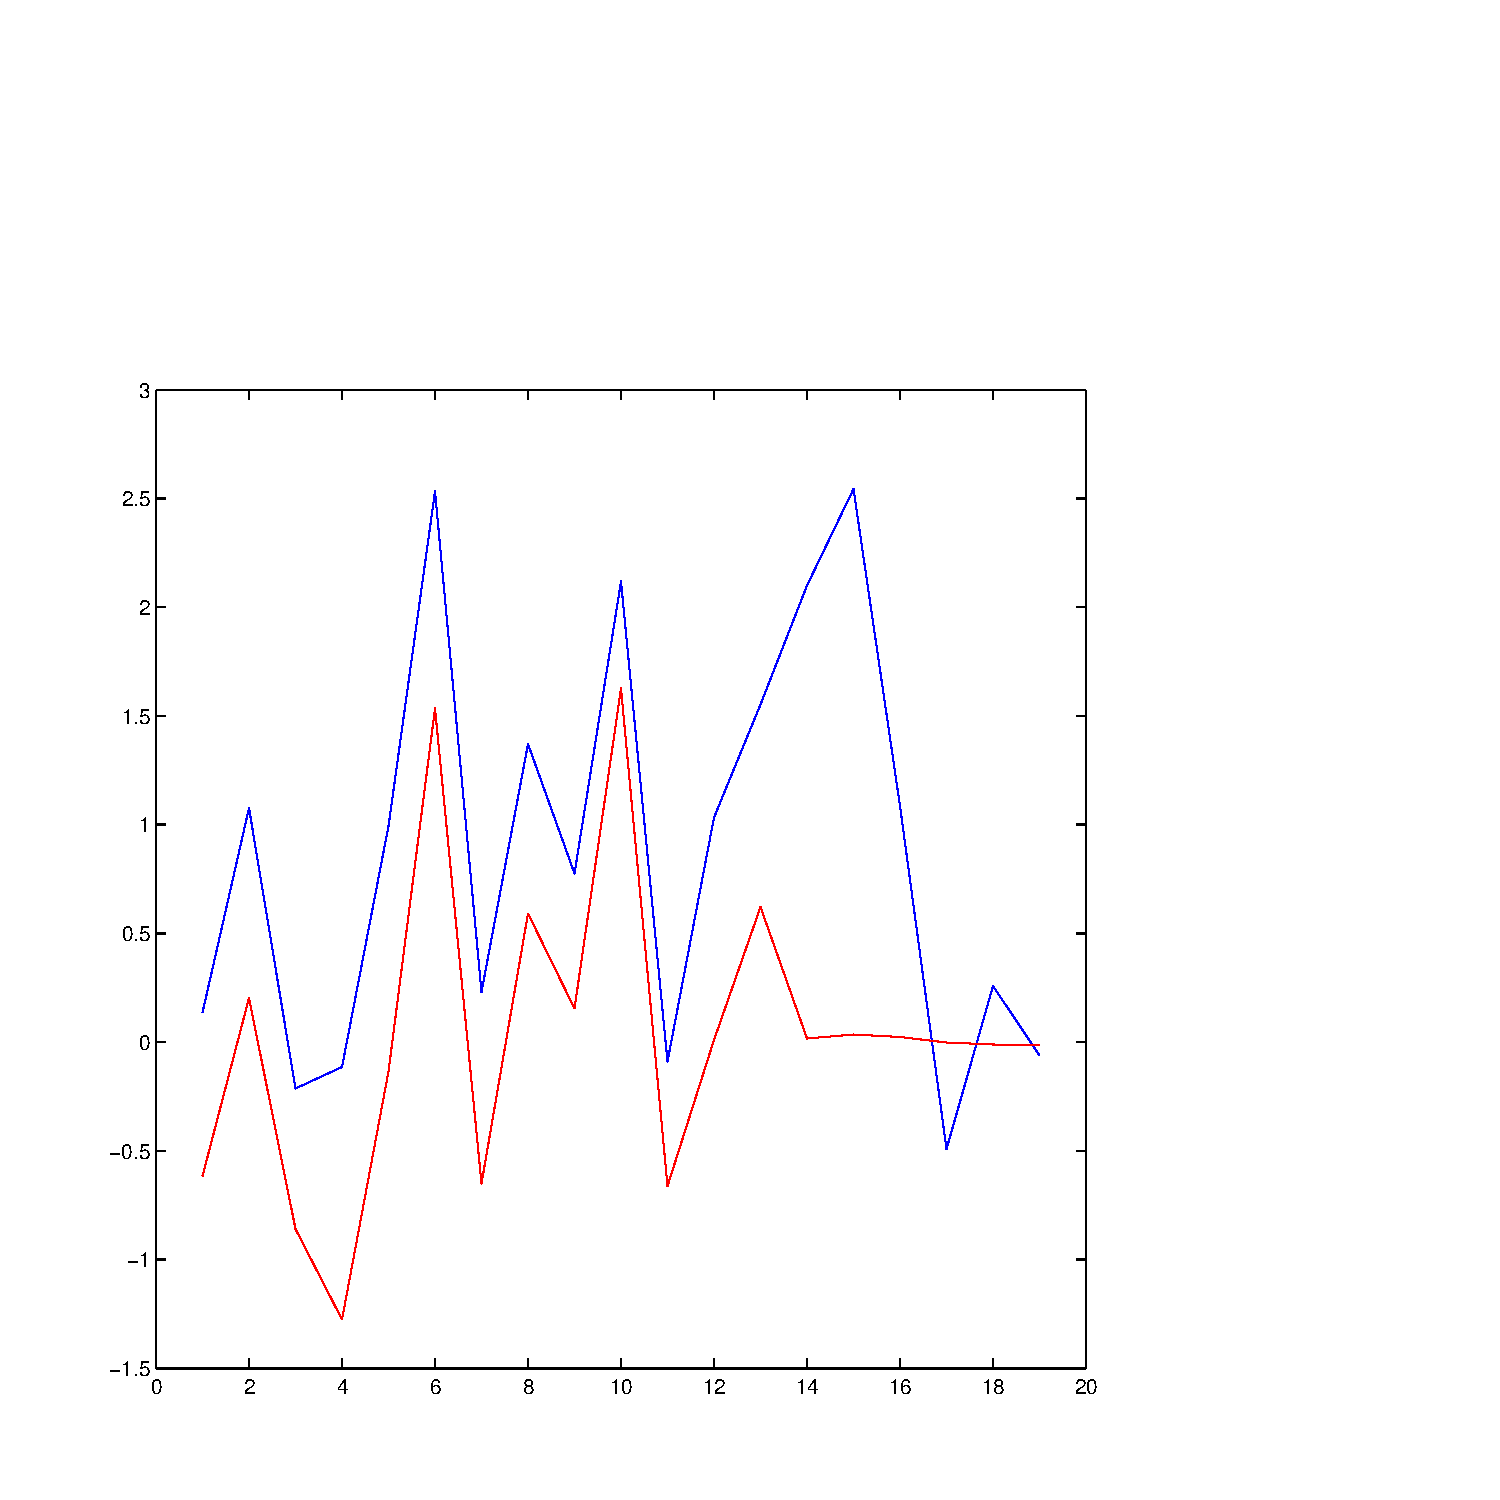
\includegraphics[scale=0.3]{ex2_test1a.pdf}
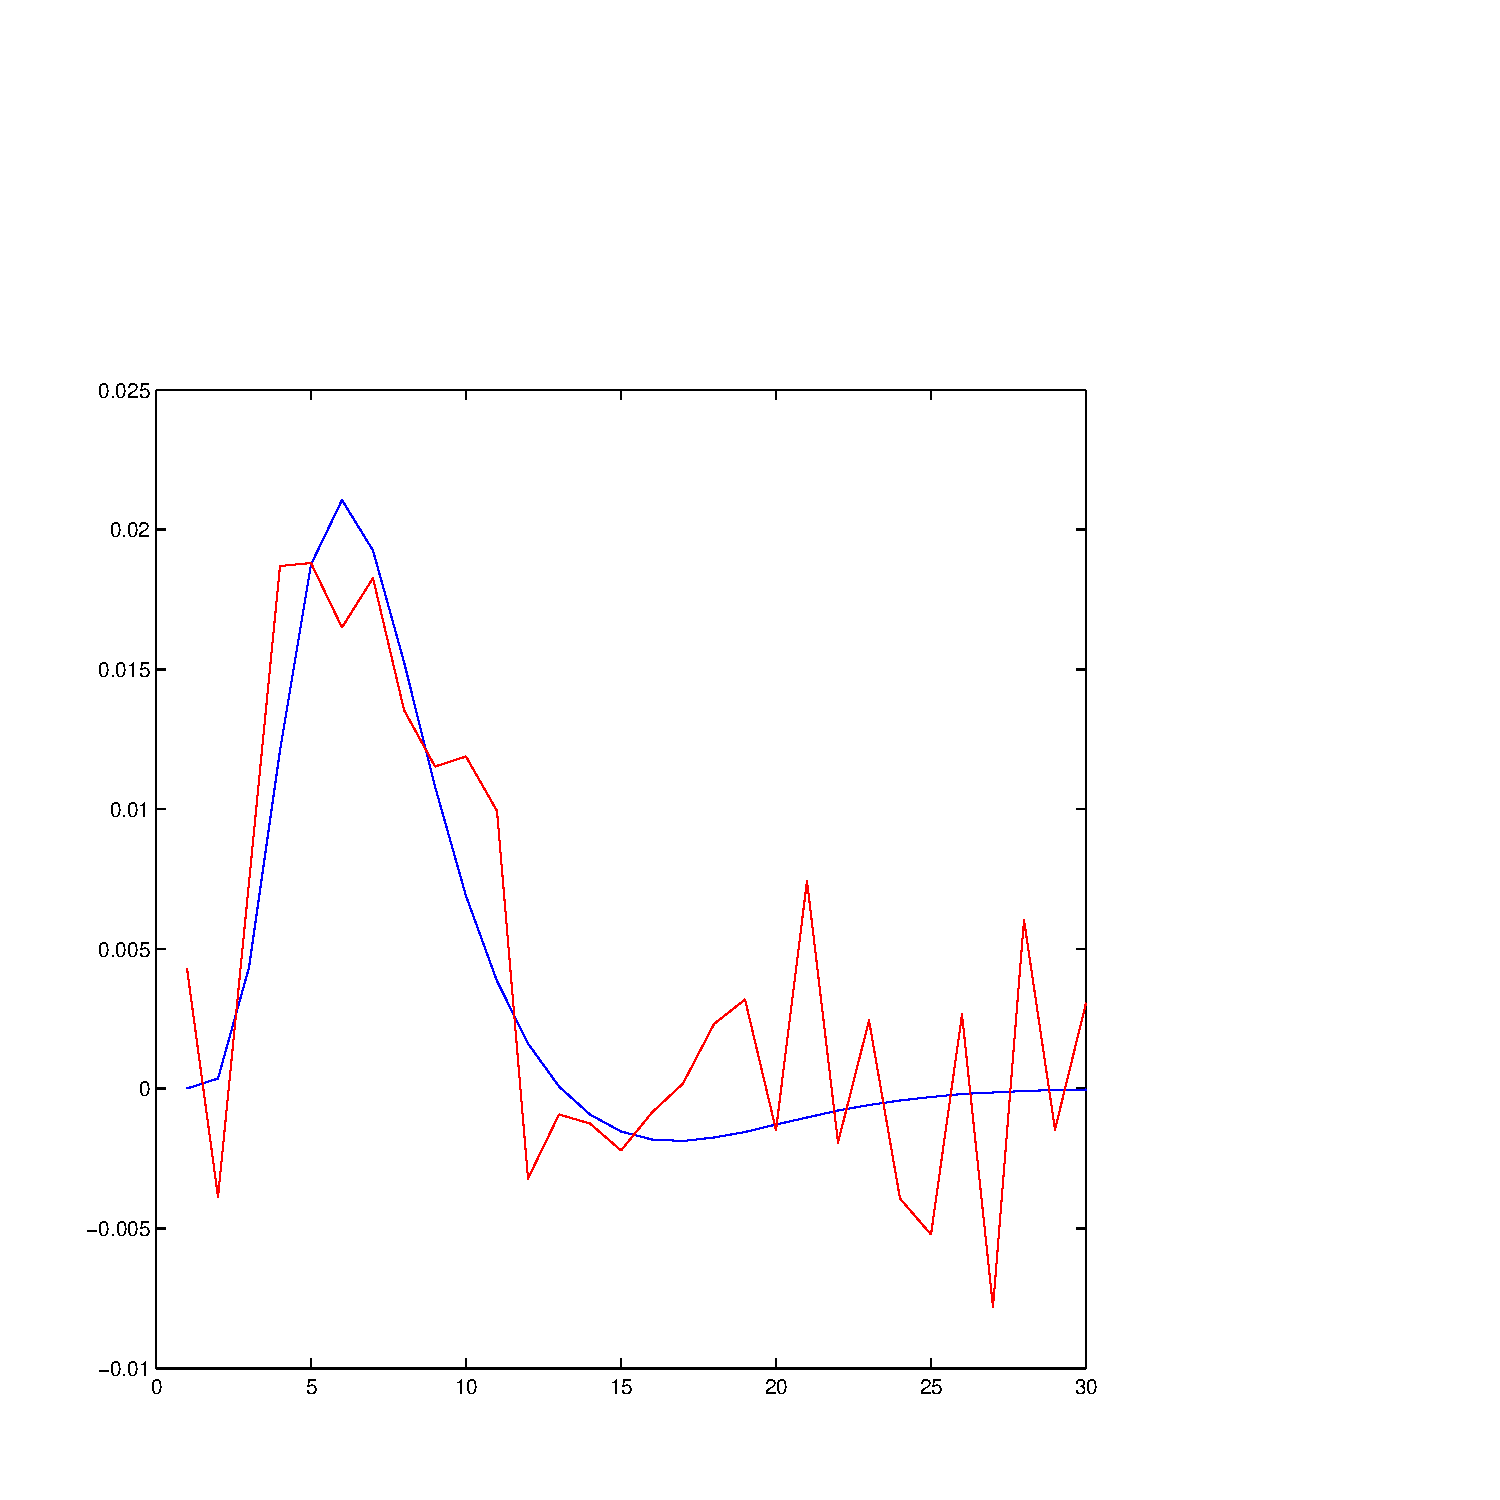
\includegraphics[scale=0.3]{ex2_test1b.pdf}
\item With regularization:
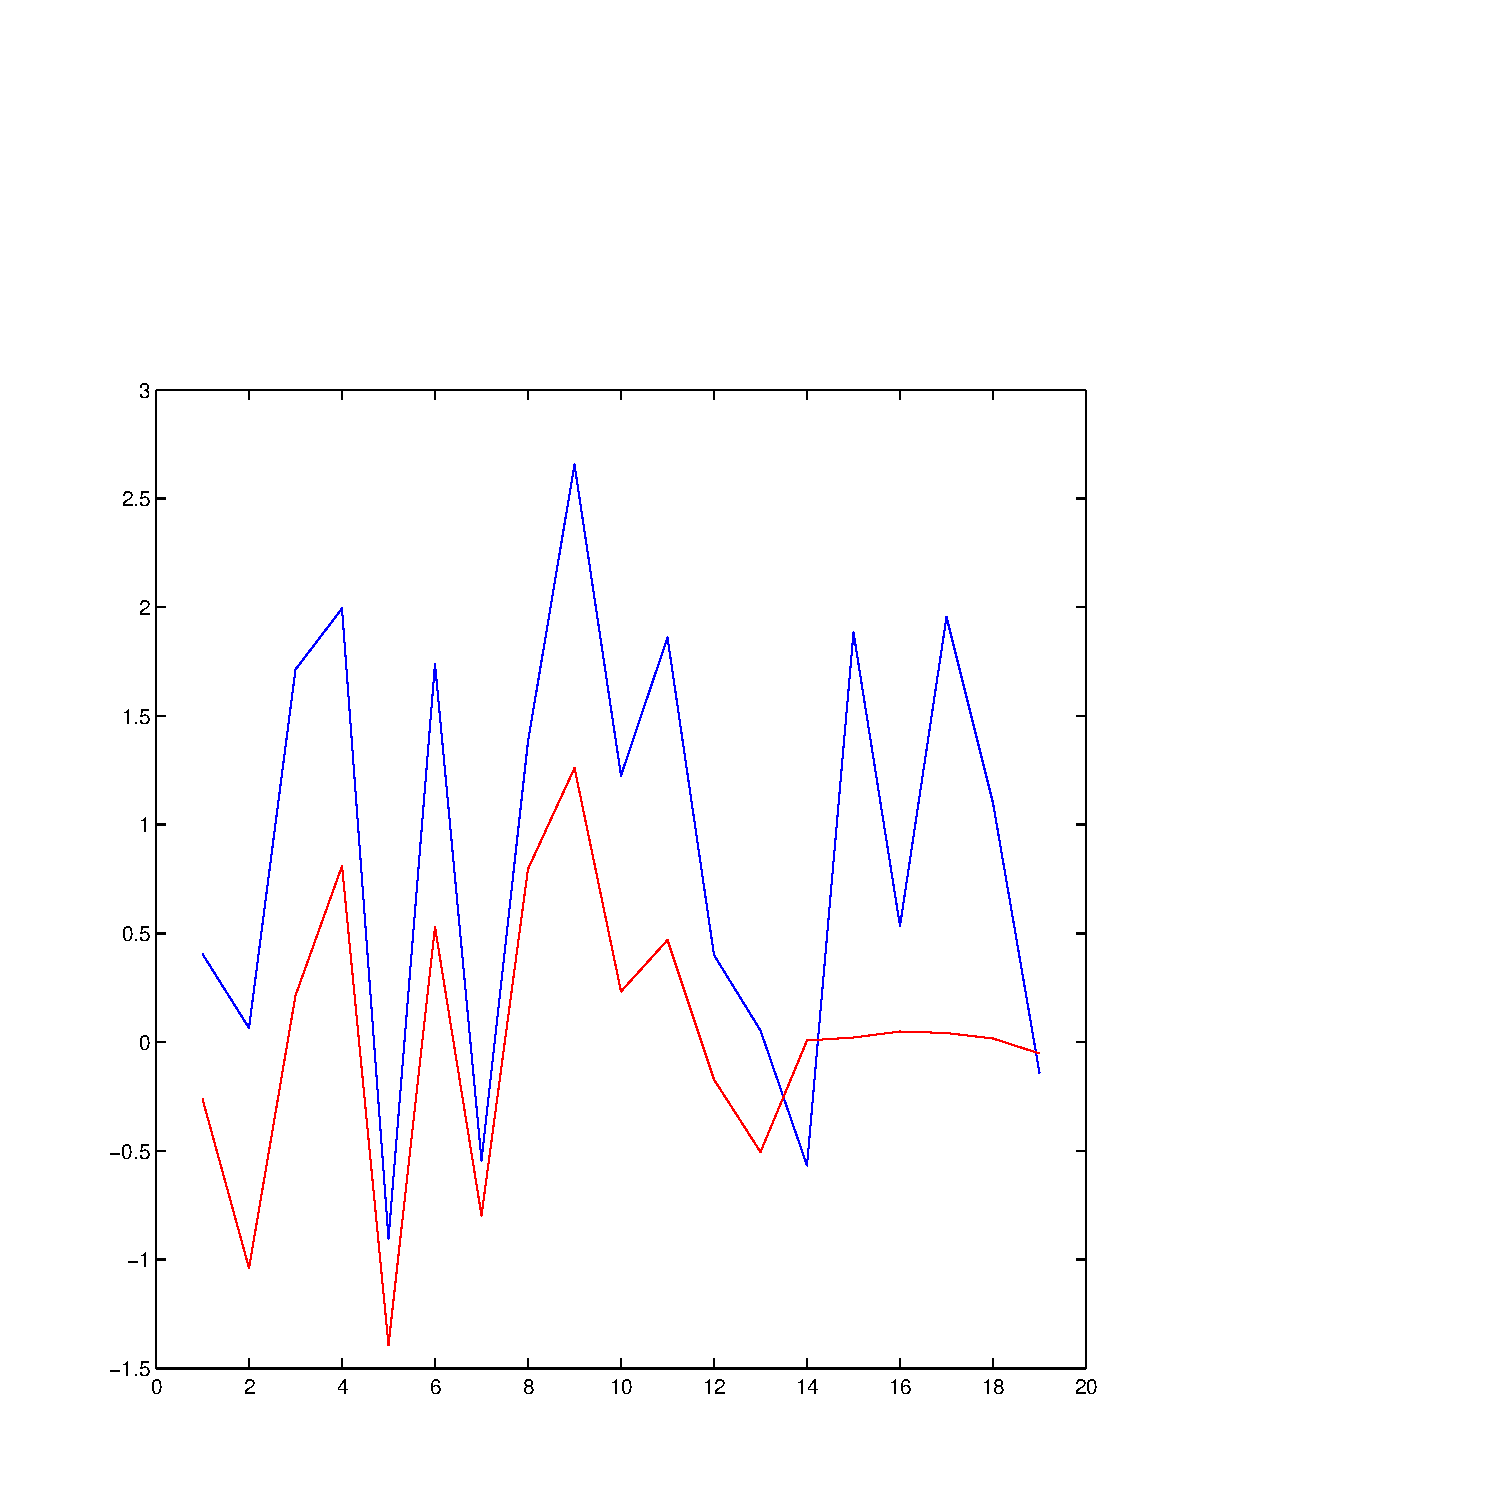
\includegraphics[scale=0.3]{ex2_test2a.pdf}
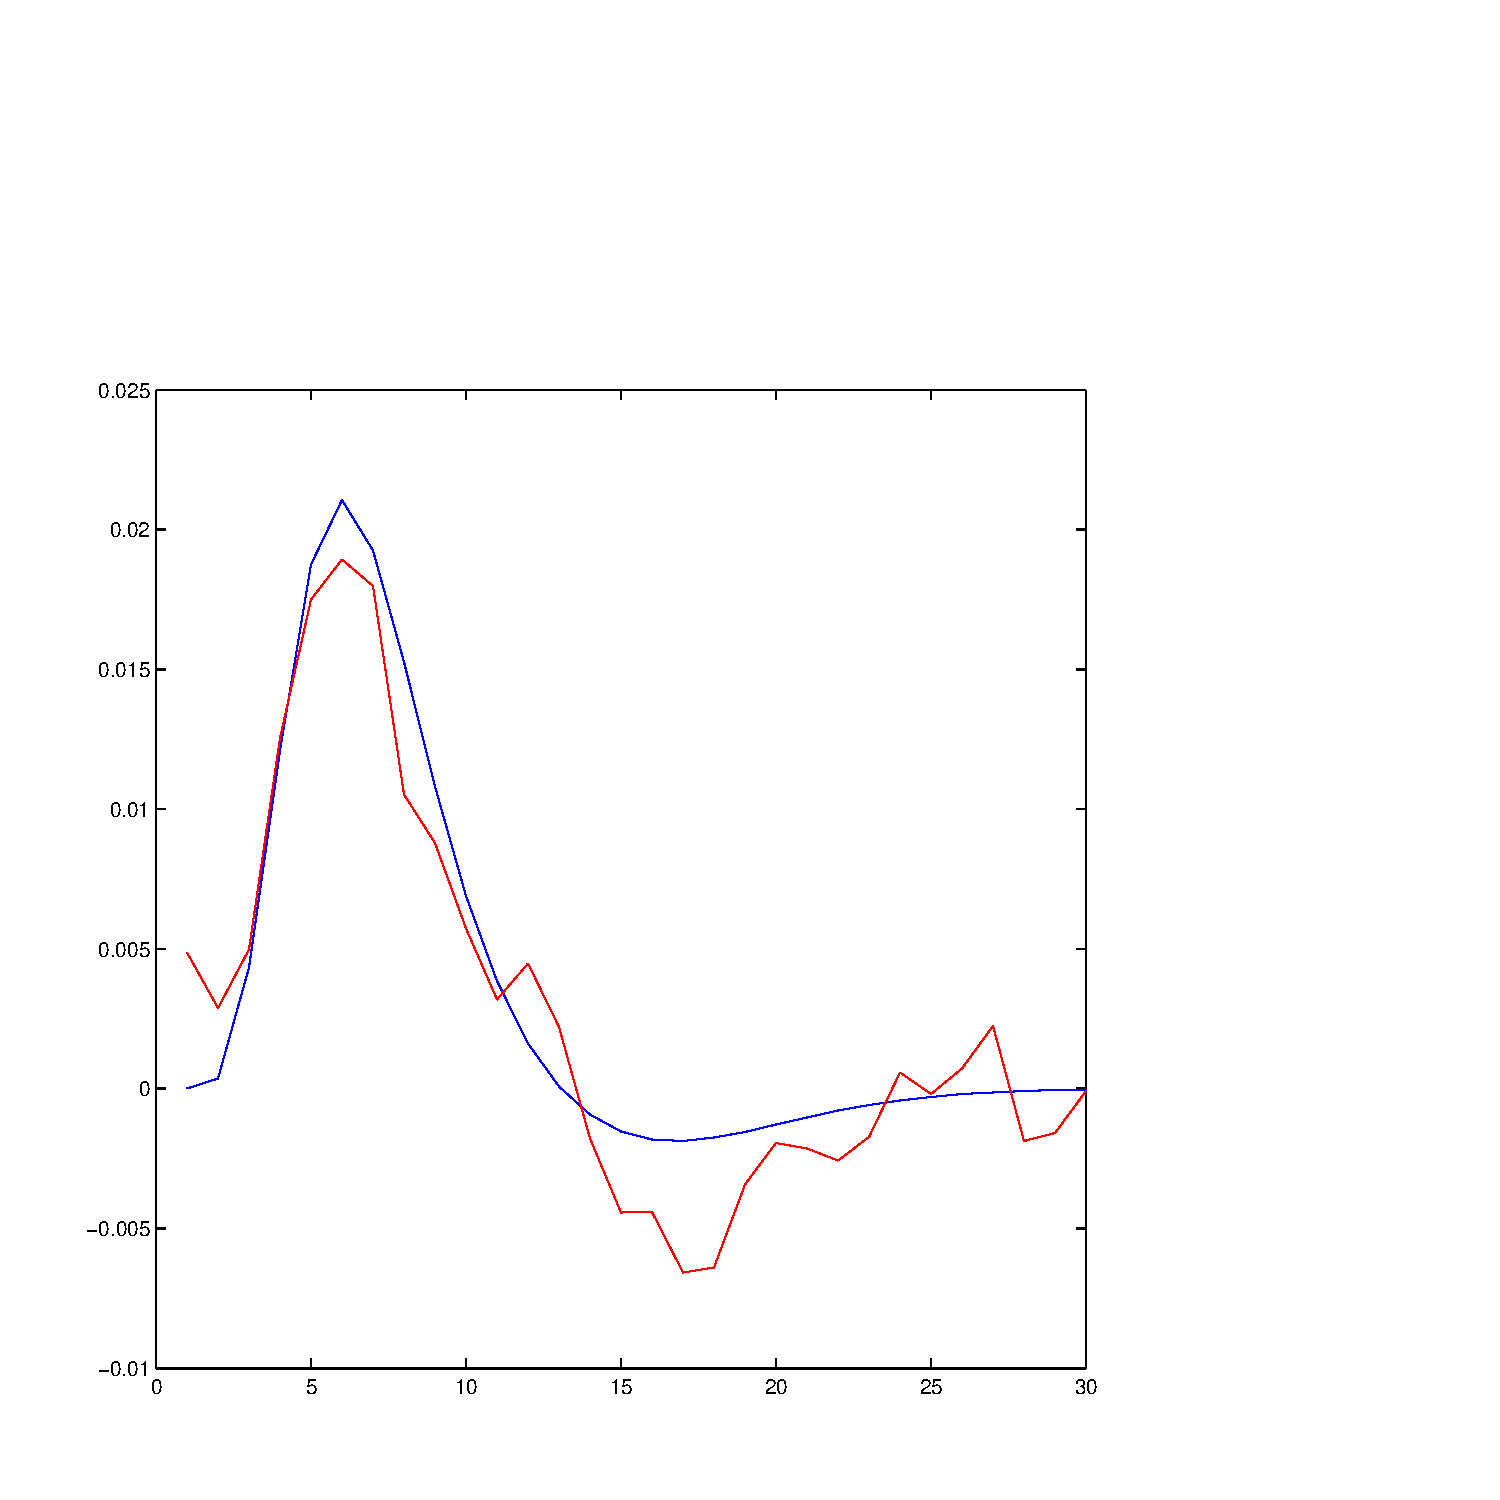
\includegraphics[scale=0.3]{ex2_test2b.pdf}
\end{itemize}
\emph{Left: amplitudes, right: HRF, blue: truth, red: estimate}
\end{frame}



\end{document}


















